\chapter[Direct Data-Driven Control (SM approach)]{Direct Data-Driven Control design: Set-Membership approach}

\vspace{-1cm}
\begin{figure}[h]
    \centering
    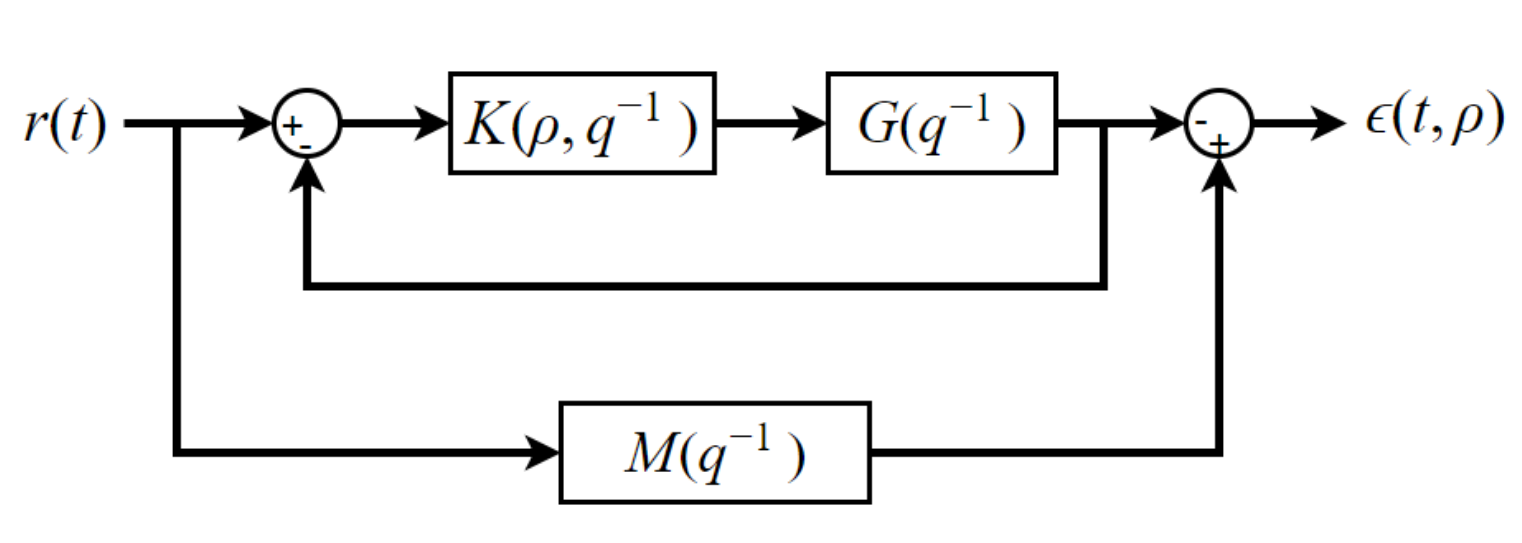
\includegraphics[scale=0.4]{img/DDDC_1.png}
    \caption{Direct Data-Driven Control (DDDC) setting}
    \label{fig:DDDC_setting}
\end{figure}

\begin{quotation}
    \noindent
    \textsf{In the previous chapter we have seen how can we build a model for a dynamical system, linear/nonlinear, SISO/MIMO. For sure, you know that one of the objective of having a mathematical model/description for a given plant is to build a certain \textit{controller} in order to modify the behaviour of the plant itself. In this chapter, going through the description of the \textit{Direct Data-Driven control problem} (DDDC), we will see how to control a certain plant without identify it, but passing directly to the controller design using data.
    }
\end{quotation}

\section{Introduction}
In the field of Control Theory there are mainly three approaches to design a controller for a given plant: 
\begin{enumerate}
    \itemsep-0.2em
    \item \textit{Model-Based technique} in which we have a model for the plant to control, and the problem is solved using some control technique according to the specific problem we have to solve (requirements based, optimal control...);
    \item \textit{Undirect Data-Driven} here since we do not have a model for the plant, at first we retrieve a model  for the plant to be controlled (using some SysId technique), then using the obtained model, some control technique is applied; 
    \item \textit{Direct Data-Driven} Here we have that the controller is designed skipping the plant identification stage, so data are used to build a model directly for the controller.
\end{enumerate}

In particular here the objective, with reference to the \Cref{fig:DDDC_setting} is to design the controller $K$ such that the \textbf{controlled system} could match as well as possible the behaviour of the \textbf{reference model} $M$. In particular given $K(\rho, q^{-1})$, $\rho$ is the \textit{parameter vector} defined as
\begin{equation}
    \rho=[\rho_1 \quad \rho_2 \quad \dots \quad \rho_{n_\rho}]
\end{equation}
\noindent
and we want that 
\begin{equation}\label{eq:approxim}
    T_{ry}(q^{-1})=\frac{G(q^{-1} K(q^{-1}))}{1+G(q^{-1} K(q^{-1}))} \approx 
M(q^{-1})
\end{equation}
Both $K$ and $G$ are assumed to be LTI dynamical systems and the description of $G$ is not available, that is there is no model for the plant to  be controlled. From now on we will assume $M=M(q^{-1})$, $G=G(q^{-1})$ and $K=K(q^{-1})$

\section{Ideal controller $K^*$}
Ideally we want that the \Cref{eq:approxim} could hold with the equality so that
\begin{equation}\label{eq:MMP}
    M=\frac{KG}{1+KG}
\end{equation}
which is the so called \textbf{model matching problem}. We have said that $G$ is not known, but assume for a moment that we are able to know exactly $G$. In this case the model matching problem has a \textit{trivial solution} which corresponds to obtaining an \textbf{ideal controller} $K^*$. By doing simple algebraic manipulation we obtain

\begin{equation}
    M=\frac{GK}{1+GK} \iff M+MGK=GK \iff KG(1-M)=M \iff K^*=\frac{M}{G(1-M)}
\end{equation}
Such a $K^*$ has interesting theoretical property useful in order to go on the description of the DDDC problem, however it can be easily shown that: 
\begin{enumerate}
    \itemsep-0.2em
    \item The resulting $K^*$ from algebraic computations can be \textit{not physically realizable}, using such a trivial formula you are not sure that
    \begin{equation*}
        \deg(D_{K^*}) \ge \deg(N_{K^*}) 
    \end{equation*}
    \item $K^*$ is not guaranteed to provide internal stability of the feedback control system\footnote{
        Remember that an DT LTI Feedback control system is stable if: 
        \begin{itemize}
            \itemsep-0.2em
            \item All of the roots of $1+L(z)$ belongs to the \underline{open unit circle}
            \item No unstable zero-pole cancellations occurs when $L()z$ is formed.
        \end{itemize}
    }, since there can be \textit{unstable zero-pole cancellations}.
\end{enumerate}

\noindent
It can be easily prooved that if we include all of the unstable zeros of $G(q^{-1})$ in the reference model $M(q^{-1})$ then $K^*$ computed is ensuring internal stability of the FCS. But this way you have to pay something: if $M$ (how we will see) is obtained by using some performance requirements, including such new zeros in it will result in a non accurate description of the desired I/O behaviour! We have to derive the controller using a \textbf{different approach}.

\section{Formulation of the DDD control problem}
We wonder here how to solve the model-matching problem when: i) $G(q^{-1})$ is not known, (ii) we can collect I/O data by performing an \textit{open-loop} experiment on the plant to be controlled. Then we want to solve the problem (\ref{eq:MMP}), where $K$ is \textbf{to design}, $G$ is unknown, finally $M$ is given and retrieved taking into account some performance requirements. Going on, you can see that from \Cref{eq:MMP} you can find a \textbf{model matching error transfer function}
\begin{equation}
    E(q^{-1})=M-\frac{KG}{1+KG}
\end{equation}

\noindent
The ideal task is to \textbf{find $K$} such that $E(q^{-1})=0$, we can define the \textbf{output matching error} by multiplying both sides of \Cref{eq:MMP} by the reference $r(k)$
\begin{equation}
    \epsilon(\rho,q^{-1})=\bigg(
        M-\frac{KG}{1+KG}
    \bigg)r(k)
\end{equation}
From this you can see that if $T \approx M$ then $\epsilon(\rho, q^{-1})=0$, and 
\begin{equation}\label{eq:final}
    Mr = \frac{KG}{1+KG}r      \quad    \forall r(k) 
\end{equation}
Here the problem is that we do not have the model $G(q^{-1})$ for the plant and so we cannot find properly the controller $K(\rho, q^{-1})$! How can we go ahead? If we better analyze the \Cref{eq:final} we can exploit a useful insight, in fact
\begin{equation}\label{eq:dddc1}
    Mr-MKGr = KGr \iff (1-M)KGr = Mr \iff KGr(k) = \frac{M}{1-M} r(k)
\end{equation}
Here we have that tber term $Gr(k)$, is by definition equal to the (noise-free) output $y(k)$ of the plant $G$ when you apply the reference signal $r(k)$. The left hand side term is a signal obtained (by simulation) obtained by filtering $r(k)$ by using the transfer function $M/(1-M)$, we can call
\begin{equation}
    s(k)=\frac{M}{1-M}r(k) 
\end{equation}
Then the \Cref{eq:dddc1} can be written as:
\begin{equation}\label{eq:dddc2}
    \Large
    \color{red}
    K(\rho,q^{-1}) y(k) = s(k)
\end{equation}
We can notice that \Cref{eq:dddc2} is formulating a System Identification problem. We want to find $K$, and so its parameters $\rho$ given the input $y(k)$ and the output $s(k)$, where: 
\begin{itemize}
    \itemsep-0.3em
    \item $y(k)$ are the noise free samples of the output of the plant $G$ when the reference signal $r(k)$ is applied as input. Note that since we perform an experiment, we collect noisy data, then you must use
    \begin{equation}
        y(k)=\tilde{y}(k)-\eta(k)
    \end{equation}
    \item $s(k)$ are the samples obtained by stimulating (in simulation) the model $M/(1-M)$ with the reference signal $r(k)$.
\end{itemize}
Finally, we have
\begin{equation}\label{eq:dddc3}
    K(\rho,q^{-1}) [\tilde{y}(k)-\eta(k)] = s(k)
 \end{equation}
that is an \textbf{Input-Error} Set-Membership identification problem where the noise samples are assumed to be UBB (Unknown but bounded), so that
\begin{equation}
    \vert \eta(k) \vert \le \Delta_\eta
\end{equation}

\begin{remark}
    Note that from the development of the theory the following three conditions are equivalent:
    \begin{itemize}
        \itemsep-0.3em
        \item $E(q^{-1})=0$
        \item $\epsilon(\rho,q^{-1})=0$
        \item $K(\rho,q^{-1})r(k)=M (1-M)^{-1} r(k)$
    \end{itemize}
\end{remark}

\section{Set-Membership approach to DDDC (SM-DDDC)}
Now, we have started from the model matching problem, by using some simple algebraic manipulations we have obtained the \textit{output-matching error}, finally we have formulated the problem of designing a controller in the form given by \Cref{eq:dddc3}. Here the objective is to explore how we can formulate a feasible set for the solutions of the problem, and how can be formulated the uncertainty intervals for the parameters describing the controller. It is noticeable that the Input-Error SM-ID problem is a particular case of the Error-In-Variables one! Nothing new, except for the focus we have in this chapter.\\

\noindent
In order to solve the SM-ID problem we need to select the controller class $\mathcal{C}$. For example, this is the same to decide: 
\begin{enumerate}
    \itemsep-0.3em
    \item $\mathcal{C}$=\{class of PID controllers\}
    \item $\mathcal{C}$=\{class of LTI controllers  of fixed and given order $n$\}
\end{enumerate}

How we are going to see in a minute, this framework is providing us a sistematic way to check that the choosen class $\mathcal{C}$ is suitable or not. But first, we introduce also here the equivalent of the feasible parameter set on which is based the SM approach.

\subsection{Feasible Feasible Controller Parameter Set (FCPS)}
Here the parameters that the SM procedure outputs are referred to the controller $K(\rho,q^{-1})$, so we are seeking for a \textbf{Feasible Controller Parameter Set (FCPS)}. In general this can be written as: 
\begin{equation*}
    \begin{aligned}
        \mathcal{D}_\rho=&\{
        \rho\in\mathbb{R}^{n_\rho} \ : s(k)=K(\rho,q^{-1})[\tilde{y}(k)-\eta(k)]\\
        &\vert \eta(k) \vert \le \Delta_\eta \quad k=1,...,N 
    \}
    \end{aligned}
\end{equation*}
In order to give an example we can assume that $\mathcal{C}=\{\text{class of first order LTI controllers}\}$, in this way we have a closed form for $K(\rho,q^{-1})$:
\begin{equation}
    K(\rho,q^{-1})=\frac{\rho_2+\rho_3q^{-1}}{1+\rho_1 q^{-1}}
\end{equation}
In this way the FCPS becomes ($n_\rho=3$): 
\begin{equation}
    \begin{aligned}
        \mathcal{D}_\rho=&\{
        \rho\in\mathbb{R}^3: s(k) + \rho_1 s(k-1) -\rho_2 \tilde{y}(k)\\
        &-\rho_3 \tilde{y}(k-1) + \rho_2 \eta(k) + \rho_3 \eta(k-1)=0 \quad k=2,...,N\\
        &\vert \eta(k) \vert \le \Delta_\eta \quad k=1,...,N
    \}
    \end{aligned}
\end{equation}

We know that there is no way to eliminate the dependence on the noise samples $\eta(k)$, fir this reason we have to extend the FCPS into an \textit{Extended Feasible Controller Parameter Set} (EFCPS) $\mathcal{D}_{\rho,\eta}$, defined by: 

\begin{equation}
    \begin{aligned}
        \mathcal{D}_{\rho,\eta}=&\{
        \rho\in\mathbb{R}^3, \ \eta \in \mathbb{R}^N: s(k) + \rho_1 s(k-1) -\rho_2 \tilde{y}(k)\\
        &-\rho_3 \tilde{y}(k-1) + \rho_2 \eta(k) + \rho_3 \eta(k-1)=0 \quad k=2,...,N\\
        &\vert \eta(k) \vert \le \Delta_\eta \quad k=1,...,N
    \}
    \end{aligned}
\end{equation}

If at this stage $\mathcal{D}_{\rho,\eta}$ is \textbf{empty} than, there is no controller in the considered class $\mathcal{C}$ which solves the control problem. This is an evidence that the EFCPS is giving us a tool by which we can check if we have correctly chosen the controller class. \\
Moreover, it holds that $\mathcal{D}_{\rho, \theta}=\varnothing $ if and only if at least one of the POP to be solved for computing the \textbf{Controller Parameter Uncertainty Intervals (CPUIs)} has \texttt{exitflag}<0. 

\subsection{Summarizing the $K(\rho,q^{-1})$ design procedure}
In order to \textbf{design a Direct Data-Driven controller (DDDC)} $K(\rho,q^{-1})$: 
\begin{enumerate}
    \itemsep-0.3em
    \item Perform an open-loop experiment by applying $r(k)$ to the plant to be controlled and collect the output $\tilde{y(k)}=y(k)+\eta(k)$, with $\eta(k)$ bounded; 
    \item Build the Feasible Controller Parameter set and Extended Feasible Controller Parameter Set ($\mathcal{D}_{\rho}$ and $\mathcal{D}_{\rho,\eta}$).
    \item Compute the \textit{Controller Parameter Uncertainty Intervals}:
    \begin{equation}
        CPUI_{\rho_i}=[\underline{\rho}_i, \overline{\rho}_i] \quad 
        \underline{\rho}_i= \min_{\rho,\eta \in \mathcal{D}_{\rho,\eta}} \rho_i \quad
        \overline{\rho}_i= \max_{\rho,\eta \in \mathcal{D}_{\rho,\eta}} \rho_i 
    \end{equation}
    \vspace{-0.2cm}
    \item Two sitautions can occur at this point:
    \vspace{-0.3cm}
    \begin{itemize}
        \itemsep-0.3em
        \item[a] If one of the problem is infeasible than update $\mathcal{C}$  (see\footnote{
            A possible way to proceed is the following: starting from $n=1$, FCPS is empty? YES $\to$ increase $n$; NO $to$ Ok, we are done and we can compute CPUIs!
        });
        \item[b] If all the POPs are feasible (\texttt{exitflag}>0) we obtain the CPUIs for all $rho_i$
    \end{itemize}
    \item Build the controller transfer function as:
    \begin{equation}
        K_c(\rho^c,q^{-1})=\frac{\rho^c_{n+1} + \rho^c_{n+2}q^{-1}+...+\rho^c_{2n+1} q^{-n}}
        {1+\rho_1^c q^{-1}+\rho_2^c q^{-2}+...+\rho_n^c q^{-n}}
    \end{equation}
    where
    \begin{equation}
        \rho^c =[\rho^c_1,..., \rho^c_{2n+1}] \iff \rho_i^c = \frac{\underline{\rho}_i+\overline{\rho}_i}{2}
    \end{equation}
    \noindent
    If $K^c$ belongs to $\mathcal{C}$, then the ideal controller belongs to the Feasible Controller Set
\end{enumerate}

\begin{remark}
    It can be prooved that the central estimate $\rho^c$ is the solution to the following optimization problem
    \begin{equation}
        \large
        \rho^c = \arg \min_{\rho\in\mathbb{R}^p} \max_{\rho'\in\mathcal{D}_{\rho}} {
            \Vert \rho-\rho'\Vert_\infty
        }
    \end{equation}
    this is called the \textbf{Chebychev center in the $\ell_\infty$-norm} and it is the point of minimum distance from the farthest point in the FCPS. Then this is the point guaranteeing the \textit{minimum uncertainty} which is possible.
\end{remark}

\section{Data-driven stability certification}
\textbf{Stability} is a property of paramount importance for all the feedback control systems (FCS). By definition a FCS is stable if \textit{all signals} remanin bounded when bounded inputs are applied, in other terms this implies that all of the transfer functions from any input to any output of the FCS is BIBO stable. Approaching the problem of DDDC we have seen that the problem can be recasted as an input error SM-ID problem.\\
After having chosen the dynamical order for $K$, the problem is solved and a \textbf{central controller} $K_c(\rho^c,q^{-1})$ is found. Now, an important question to be answered is the following:
\begin{center}
    \textbf{How to certify that $K^c$ stabilizes the unknown plant?}
\end{center}
In the DDDC framework, stability must be certified according to the following conditions:
\begin{itemize}
    \itemsep-0.2em
    \item The only available information of the unknown plant is the dynamical order that could be (in a conservative way) less than or equal to a given non negative integer $n_P$; 
    \item A central controller $K_c$ has been obtained at this stage;
    \item A set of input-output data collected on the plant is available and finally the output measurements are affected by Unknown-but-bounded (UBB) noise.
\end{itemize}

Uncertainty on data makes the problem of certifying stability harder, since the stability must be provided for \textbf{all allowed realizations} of the noise within the specified bound. Due to the presence of such uncertainty, some key ideas from \textit{robust control framework} are used, with the only difference that our focus here is \underline{not} on an uncertain description of the plant, but on an uncertain description of the controller $K$ that has been obtained by using I/O noisy data.

\subsection{Background concepts}

\subsubsection{$\mathcal{H}_\infty$-norm}
In the framework of $\mathcal{H}_\infty$ robust control, a controller $G_c$ which fulfills robust stability and nominal performance requirements is designed. The optimization objective are given in term of $\mathcal{H}_\infty$-norm whose definition is given in the following: 
\begin{definition}[\textsf{$\mathcal{H}_\infty$-norm}]
    Consider a transfer function $G(z)$, the $\mathcal{H}_\infty$-norm of $G(z)$ is defined as
    \begin{equation}
        \Vert G(z) \Vert_\infty \doteq \sup_{\omega\in[0,2\pi]} {\vert G(e^{i\omega})} \vert
    \end{equation}
\end{definition}
\noindent
Roughly speaking this is the maximum amplification of the $G$ input's energy.

\subsubsection{Small-gain theorem}

\begin{multicols}{2}
    \begin{figure}[H]
        \centering
        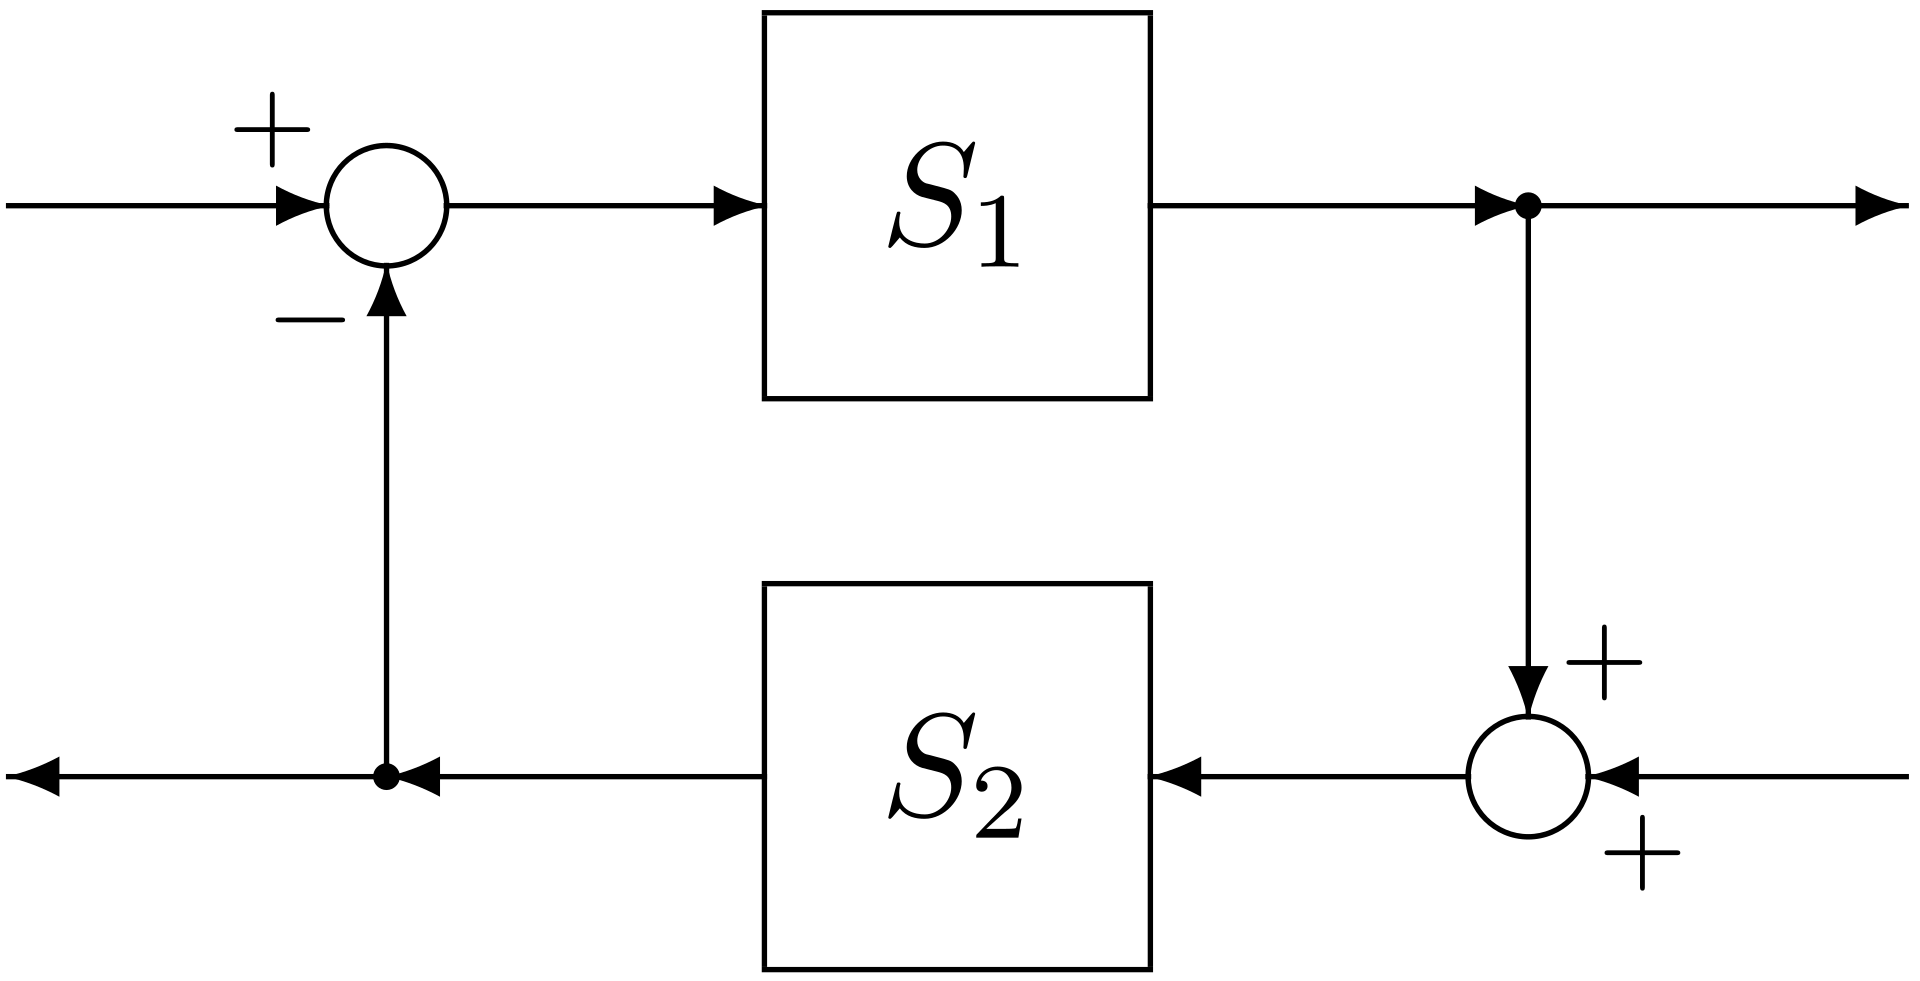
\includegraphics[scale=0.12]{img/small_gain.png}
    \end{figure}
    
    \begin{theorem}[Small-Gain Theorem]
        Suppose $S_1$ and $S_2$ are stable. Then, the interconnected system shown in the figure is well-posed and internally stable if and only if 
        \begin{equation}
            \Vert S_1 S_2 \Vert_\infty < 1
        \end{equation}
 \end{theorem}
    \noindent{
        \small{
            \textsf{See \Cref{p:Appendix}, \Cref{ch: SMT_example} for an example.}
        }
    } 
    
\end{multicols}

\subsection{Small-gain theorem in DDDC}
Since the plant is unknown, any attempt to describe the uncertainty affecting the plant leads to an \textbf{indirect data-driven control} problem. As we gave anticipated we describe the uncertainty as if it was on the controller and in particular: the \textit{ideal controller $K$*} plays the role of the nominal plant, while the uncertainty is given by the \textit{distance between the actual and ideal controller}.

\begin{figure}
    \centering
    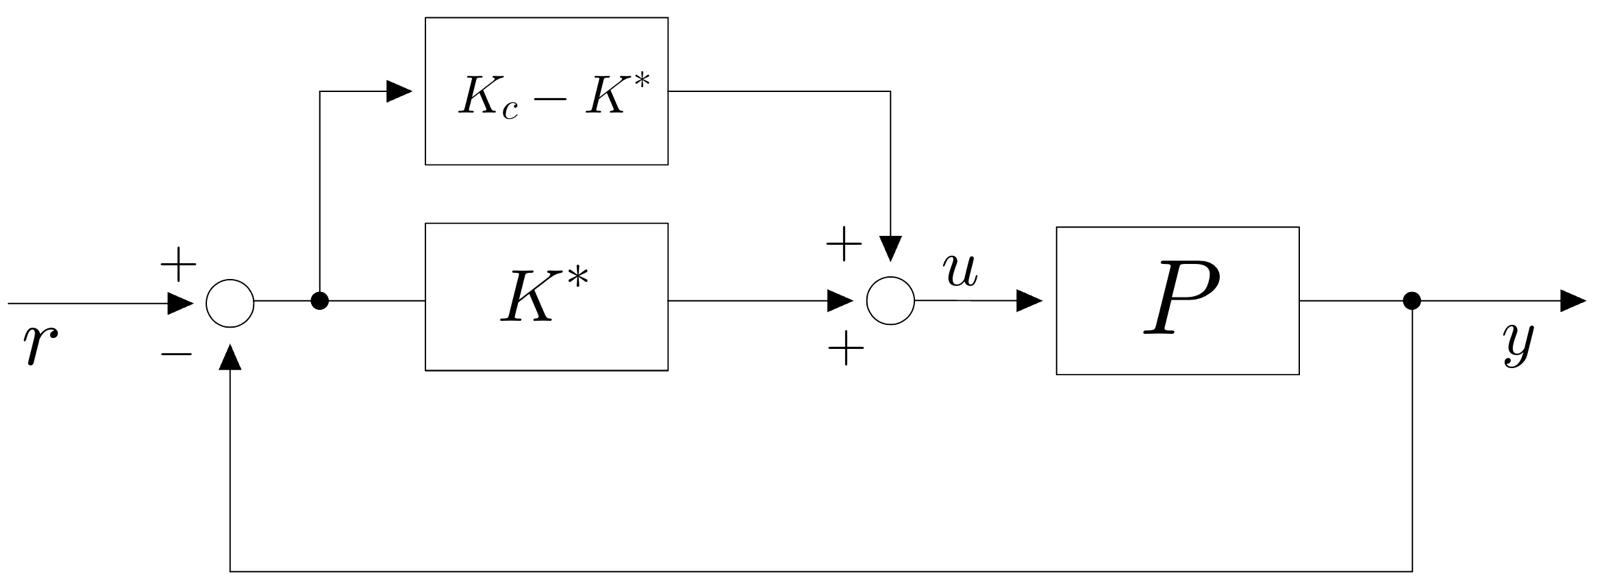
\includegraphics[scale=0.25]{img/SMT_DDDC.jpg}
    \caption{Uncertain description of the controller}
\end{figure}

\noindent
In this context the \textit{Small-gain theorem} can be applied where the subsystems $S_1$ and $S_2$ are defined as:
\begin{equation}
    S_1 = K_c-K^*, \quad S_2=\frac{-P}{1+K^*P}
\end{equation}
The following important theorem is given (whose proof can be retrieved from \cite{van2011data}):
\begin{theorem}\label{th:stab}[\Citeauthor{van2011data}, \citeyear{van2011data})]
    Let
    \begin{equation}\label{eq:def_Delta}
        \Delta(z)=M(z)-K_c(z)P(z)(1-M(z))
    \end{equation}
    the controller $K_c$ stabilizes the plant $P$ if
    \begin{enumerate}
        \itemsep-0.2em
        \item The ideal controller $K^*=\frac{M}{P(1-M)}$ stabilizes the plant; 
        \item $\Delta(z)$ is stable;
        \item $\Vert \Delta(z) \Vert_\infty<1$
    \end{enumerate}
\end{theorem}

\noindent
At this point, we can say that: (i) Condition 1 is satisfied if $M$ is stable and no unstable cancellations occur; (ii) Condition 2 is satisfied if both $P$ and $M$ are stable. But, \textbf{How to compute $\Vert \Delta(z) \Vert_\infty$ without using the plant and given noisy data?} The following section is aimed to answer to this question.

\subsection{Set-Membership estimation of $\Vert \Delta(z) \Vert_\infty$}
A three-steps procedure can be used, in order to obtain frequency by frequency a worst-case estimate on $\vert \Delta(e^{i\omega}) \vert$. 

\subsubsection{First step: a-priori information on $\Delta$}
The system $\Delta(z)$ can be generally defined as
\begin{equation}\label{eq:delta_q}
    \Delta(q^{-1}) = \frac{
        \gamma_0 + \gamma_1 q^{-1} + \dots + \gamma_{n_\Delta} q^{-n_{\Delta}}
    }{
        1+\delta_1 q^{-1} + \dots + \delta_{n_{\Delta}} q^{-n_\Delta}
    }
\end{equation}
from the definition of $\Delta$ we can say that $n_\Delta \le n_K + n_P +  n_M$, where $K, P, M$ are respectively the central controller, the plant and the reference model. Moreover using \Cref{eq:def_Delta}, and multiplying both sides by $r(k)$ you can get rid of the unknown plant
\begin{align}
    &\Delta(q^{-1}) r(k) = M(q^{-1}) r(k) - K_c(q^{-1}) (1-M(q^{-1})) 
    \overbrace{P(q^{-1}) r(k)}^{y(k)=\tilde{y}(k)-\eta(k)}\\
    &\Delta(q^{-1}) r(k) = M(q^{-1}) r(k) - K_c(q^{-1}) (1-M(q^{-1})) 
    {[\tilde{y}(k)-\eta(k)]}=\\
    &=Mr(k)-K_c(1-M)\tilde{y(k)} + K_c(1-M)\eta(k)=\\
    &=z(k) + F(q^{-1}) \eta(k) \label{eq:lastmaxdelta}
\end{align}
Here the samples of $z(k)$ can be obtained by simulation, while $F(q^{-1})$ is completely known.

\subsubsection{Second step: worst-case norm estimation problem}
For a fixed frequency $\omega$ a worst-case norm estimation can be obtained as:
\begin{equation}\label{eq:original_Delta_prob}
    \begin{aligned}
        &\max_{\Delta,\eta} \vert \Delta(e^{i\omega}) \vert\\
        &{\text{s.t.}}\\
        &\Delta(q^{-1})r(k) = z(k) + F(q^{-1})\eta(k)\\
        &\vert \eta(k) \vert \le \Delta_\eta
    \end{aligned}
\end{equation}

\subsubsection{Third step: obtaining a POP}
With a non-negligiblle effort the problem in \cref{eq:original_Delta_prob} can be recasted into a POP. At first we can note that $\Delta(e^{i\omega})$ is nothing but a complex number that can be written as
\begin{equation}\label{eq:complex}
    \Delta(e^{i\omega})=a+ib
\end{equation}
we are interested in the magnitude of such a number, that is: 
\begin{equation}\label{eq:norm}
    \vert \Delta(e^{i\omega}) \vert = \sqrt{a^2+b^2} \iff \exists{t}: t=\vert \Delta(e^{i\omega}) \vert, \ t^2=a^2+b^2
\end{equation}
The powers of the numbers $e^{ik\omega}$, $k=0,...,n_\Delta$ can be written in cartesian form as: 
\begin{equation}
    \begin{bmatrix}
        e^{in_\Delta{\omega}}\\
        \vdots\\
        e^{i2\omega}\\
        e^{i\omega}\\
        e^0\\
    \end{bmatrix}=\begin{bmatrix}
        \rho_0\\\rho_1\\\rho_2\\\vdots\\\rho_{n_\Delta}
    \end{bmatrix}+ i \begin{bmatrix}
        \sigma_0\\\sigma_1\\\sigma_2\\\vdots\\\sigma_{n_\Delta}
    \end{bmatrix}
\end{equation}
As a \textbf{function of the parameters $\gamma,\delta$} we can evaluate $\Delta(e^{i\omega})$ and estabilish a relation between $a,b,\gamma,\delta$ as:
\begin{align}
    &\Delta(z=e^{i\omega})=\frac{
        \gamma_0{e^{i{n_\Delta}\omega}}+\gamma_1 e^{i(n_\Delta-1)\omega}+\dots+\gamma_{n_\Delta-1} e^{i\omega}+\gamma_{n_\Delta}
    }{
        \delta_0 {e^{i{n_\Delta}\omega}}+
        \delta_1 e^{i(n_\Delta-1)\omega}+
        \dots + 
        \delta_{n_\Delta-1}e^{i\omega}+
        \delta_{n_\Delta}
    }=a+ib\\
    &\sum_{j=0}^{n_\Delta} \gamma_j e^{i(n_\Delta-j)\omega} = (a+ib)
    \sum_{j=0}^{n_\Delta} \delta_j e^{i(n_\Delta-j)\omega}\label{eq:dgab}
\end{align}
We have assumed that $\delta_0=1$ in order to simplify the notation. Replacing the cartesian form of the complex numbers $e^{i(n_\Delta-j)\omega}$ we obtain: 
\begin{equation}
    \sum_{j=0}^{n_\Delta} \gamma_j (\rho_j+\sigma_j) = (a+ib)
    \sum_{j=0}^{n_\Delta} \delta_j (\rho_j+\sigma_j)
\end{equation}
\noindent
By separating real and imaginary parts we obtain:
\begin{equation}
    \sum_{j=0}^{n_\Delta} \gamma_j \rho_j + i \gamma_j\sigma_j = 
    \sum_{j=0}^{n_\Delta}{
        a \delta_j \rho_j + i a \delta_j \sigma_j + i  b \delta_j \rho_j - b \delta_j \sigma_j
    }
\end{equation}
The two sides are equal if and only if the real parts are equal each other, the same for the imaginary parts, then two equations are obtained: 
\begin{align}
    &\sum_{j=0}^{n_\Delta} {\color{red}\gamma_j} \rho_j= \sum_{j=0}^{n_\Delta}{
         {\color{red}a\delta_j} \rho_j  -  {\color{red}b\delta_j} \sigma_j 
    } \quad \textsf{Real parts}\label{eq:real}\\ 
    &\sum_{j=0}^{n_\Delta} {\color{red}\gamma_j} \sigma_j= \sum_{j=0}^{n_\Delta}{
        {\color{red}a \delta_j} \sigma_j  + {\color{red}b \delta_j} \rho_j 
    } \quad \textsf{Imaginary parts}\label{eq:img}
\end{align}

\noindent
In {\color{red}red} the optimization variables, $\sigma_j$ and $\rho_j$ are known numbers. Next, $\gamma,\delta$ are related to the data and noise samples according to: $$\Delta(q^{-1}) r(k)=z(k) + F(q^{-1}) \eta(k)$$
In the following we are using  $r_k$ instead of $r(k)$ to ease the notation. Then, by using the definition of $\Delta$ and being $n_F$ and $\alpha_j^F, \ \beta_j^F$, respectively the number of parameters and the parameters of $F(q^{-1})$, we can obtain:
\begin{align}
    &\frac{
        \sum_{j=0}^{n_\Delta} \gamma_j q^{-j}
    }{
        \sum_{j=0}^{n_\Delta} \delta_j q^{-j}
    }r_k = z_k +  \frac{
        \sum_{j=0}^{n_F} \beta_j^F q^{-j}
    }{
        \sum_{j=0}^{n_F} \alpha_j^F q^{-j}
    } \eta_k \qquad \textsf{Removing the denominators...}\label{eq:first_1}\\
    &
    \bigg(\sum_{j=0}^{n_F} \alpha_j^F q^{-j}\bigg) 
    \bigg(\sum_{j=0}^{n_\Delta} \gamma_j q^{-j}\bigg) r_k=
    \bigg(\sum_{j=0}^{n_F} \alpha_j^F q^{-j}\bigg) 
    \bigg(\sum_{j=0}^{n_\Delta} \delta_j q^{-j}\bigg) r_k + 
    \bigg(\sum_{j=0}^{n_F} \beta_j^F q^{-j}\bigg) \bigg(\sum_{j=0}^{n_\Delta} \delta_j q^{-j}\bigg) \eta_k \label{eq:plain_eq} \\
    &\bigg(
        \sum_{j=0}^{n_F} \sum_{h=0}^{n_\Delta} {\alpha_j^F \gamma_h q^{-j-h}}
    \bigg) r_k =
    \bigg(
        \sum_{j=0}^{n_F} \sum_{h=0}^{n_\Delta}{\alpha_j^F \delta_h q^{-j-h}} 
        \bigg) 
    r_k+
        \sum_{j=0}^{n_F} \sum_{h=0}^{n_\Delta}{\beta_j^F \delta_h q^{-j-h}}
     \eta_k\label{eq:lastbutone}\\
     &
        \sum_{j=0}^{n_F} \sum_{h=0}^{n_\Delta} {\alpha_j^F {\color{red}\gamma_h} \ r({k-j-h})} =
        \sum_{j=0}^{n_F} \sum_{h=0}^{n_\Delta}{\alpha_j^F {\color{red}\delta_h} \ r({k-j-h})} +
        \sum_{j=0}^{n_F} \sum_{h=0}^{n_\Delta}{\beta_j^F {\color{red}\delta_h} \ \eta({k-j-h})}\label{eq:last_one}
\end{align}
A lot of boring computations have been done, in order to fix the ideas and clarify the steps, let us summarizing what we have done keeping in mind that our main focus was to obtain a POP starting from the problem in \Cref{eq:original_Delta_prob} (\textit{don't loose ourself!}):
\begin{enumerate}
    \item A generic complex number can be described by \Cref{eq:complex}, and its norm  is given by \Cref{eq:norm}, this leads to the definition of the slack variables $a,b,t$ for real and imaginary part and for the magnitude of $\Delta(e^{i\omega})$;
    \item The description of $\Delta$ has been provided in \Cref{eq:delta_q} in function of its parameters ($\gamma,\delta$), exploiting the relationship $q\to{z}$, and evaluating it in $e^{i\omega}$ we have obtained the \Cref{eq:dgab} which relates $a,b,\gamma,\delta$. In order to complete this first block of transformation, equations \cref{eq:real} and \cref{eq:img} have been obtained; 
    \item Exploiting the expression of $\Delta(q^{-1})$ in \Cref{eq:delta_q} and using the final step \cref{eq:lastmaxdelta} we can obtain a relation between $\gamma,\delta$ and the collected data $\{r_k,\tilde{y}_k\}$; 
    \item This leads to the equation \Cref{eq:first_1} in which we have put everything together and in order to unify the notation we have expressed also $F(q^{-1})$ in function of its parameters ($\alpha^F, \beta^F$); 
    \item Multiplying both sides for the denominators of a term and the other the expression in \cref{eq:plain_eq} has been obtained. To collect all the terms involving the backward-shift operator nested summations are used in \Cref{eq:lastbutone} step; 
    \item The backward-shift operator property has been applied in order to obtain the \Cref{eq:last_one}, which relates the parameters of the $\Delta(q^{-1})$ with the experimentally collected data. To conclude note that all of the parameters of F($q^{-1}$) can be easily obtained since both $K_c$ and $M$ are also known at this stage.
 \end{enumerate}

We are ready! Overall, the optimization problem is recast to:

\begin{equation}\label{eq:final_problem}
    \begin{aligned}
        &\max_{t,a,b\in\mathbb{R}, \gamma\in\mathbb{R}^{n_\Delta+1}, 
    \delta\in\mathbb{R}^{n_\Delta}, \eta\in\mathbb{R}^N} {t}\\
    &\text{s.t.}\\
    &t^2=a^2+b^2\\
    &\sum_{j=0}^{n_\Delta} {\color{black}\gamma_j} \rho_j= \sum_{j=0}^{n_\Delta}{
        {\color{black}a\delta_j} \rho_j  -  {\color{black}b\delta_j} \sigma_j 
   }\\
   &\sum_{j=0}^{n_\Delta} {\color{black}\gamma_j} \sigma_j= \sum_{j=0}^{n_\Delta}{
       {\color{black}a \delta_j} \sigma_j  + {\color{black}b \delta_j} \rho_j 
   }\\
   &\sum_{j=0}^{n_F} \sum_{h=0}^{n_\Delta} {\alpha_j^F {\color{black}\gamma_h} \ r_{k-j-h}} =\\
        &=\sum_{j=0}^{n_F} \sum_{h=0}^{n_\Delta}{\alpha_j^F {\color{black}\delta_h} \ r_{k-j-h}} +
        \sum_{j=0}^{n_F} \sum_{h=0}^{n_\Delta}{\beta_j^F {\color{black}\delta_h} \ \eta_{k-j-h}}\\
    &\vert \eta(k) \vert \le \Delta_\eta
    \end{aligned}
\end{equation}

By solving this problem by using convex SDP relaxation a bound on the true $\vert\Delta(e^{i\omega})\vert$ can be found. Theoretically since at the end we have to find an $\mathcal{H}_\infty$-norm, the problem (\ref{eq:final_problem}) must be solved for all $\omega\in[0,2\pi]$. Alternatively, to simplify an already complicated problem, we can introduce a Lipshitz continuity assumption on $\vert \Delta(e^{i\omega})\vert$, assuming that it does not increase or decay faster than a certain $L_b=100$dB/dec or $L_b=200$dB/dec. Finally, after having computed the bound on a certain number of frequencies, you take the max, such a value gives you an estimate of the searched quantity $\Vert \Delta(z) \Vert_\infty$. For more details you can refer to the paper \cite{abuabiah2023non}.\\

\noindent
To conclude this discussion, \textit{What if the Condition 3 of the \Cref{th:stab} is not satisfied?} A possible way to solve this problem is to collect a larger amount of experimental data so that the size of the FCPS is reduced. In this way the distance between the central estimate and the ideal controller becomes smaller, and in turn, $\Vert \Delta \Vert_\infty$ decreases.


\section*{References}
\begin{itemize}
    \itemsep-0.3em
    \item[\Large{\ding{45}}]  \Citeauthor{cerone2017direct}, \textit{\citetitle{cerone2017direct}}, \citedate{cerone2017direct}
    \item[\Large{\ding{45}}]  \Citeauthor{abuabiah2023non}, \textit{\citetitle{abuabiah2023non}}, \citedate{abuabiah2023non}
    \item[\Large{\ding{45}}]  \Citeauthor{van2011data}, \textit{\citetitle{van2011data}}, \citedate{van2011data}
\end{itemize}






